% high IPC realization
%
%\documentclass[10pt,twocolumn,dvips]{article}
\documentclass[10pt,dvips]{article}
\usepackage[english]{babel}
\usepackage{epsfig}
%
%\usepackage{fancyheadings}
%\usepackage[T1]{fontenc}
%\usepackage[latin1]{inputenc}
%
%\usepackage{twocolumn}
%\usepackage{verbatim,moreverb,doublespace}
%\usepackage{rotate,lscape,dcolumn,array,rotating,latexsym}
%
%\input{epsf}
%
\textwidth 6.5in
\textheight 9.0in
\topmargin -0.6in
\oddsidemargin 0mm
\evensidemargin 0mm
%
%\pagestyle{empty}
%
\begin{document}
\parskip 2mm
%
%
\title{Realizing High IPC Through a Scalable Memory-Latency Tolerant
Multipath Microarchitecture}
%
\author{
A. Khalafi, D. Morano, D.R. Kaeli\\
Northeastern University\\
{akhalafi, dmorano, kaeli}@ece.neu.edu\\
\and
A.K. Uht \\
University of Rhode Island\\ uht@ele.uri.edu
}
%
\maketitle
\thispagestyle{empty}
%
\begin{abstract}
This paper explores a microarchitecture that achieves high execution
performance on conventional single-threaded program codes without
compiler assistance.  Microarchitectures that can have several hundreds
of instructions simultaneously in execution can provide a means to extract
larger amounts of instruction level parallelism, even from programs
that are very sequential in nature.  However, several problems are
associated with such microarchitectures.
Among these are scalability issues, speculative
control flow issues, and the memory latency problem.

We present a basic overview of our microarchitecture and how it
addresses the problem of scalability with respect to the
number of instructions that can be executing.  We also discuss how we use
multipath execution to try and address the problem of mispredicted
conditional branches.  We provide simulation results for several
geometries of our microarchitecture that illustrate how higher IPC
can be realized from integer programs.  We also present
data that shows the positive effects of applying multipath execution to
the same programs.  Finally, we present data that shows the
tolerance of the microarchitecture to
high memory latency.
\end{abstract}
%
\section{Introduction}
%
A number of studies into the limits of instruction level 
parallelism (ILP) have
been promising in that they have shown that there is 
a significant amount of parallelism within
typical sequentially oriented single-threaded programs
(e.g., SpecInt-2000).  
The work of researchers like
Lam and Wilson ~\cite{Lam92},
Uht and Sindagi ~\cite{Uht95},
Gonzalez and Gonzalez ~\cite{Gon97}
have shown that there exists a great amount of instruction level
parallelism (ILP) that is not being exploited by any existing
computer designs.
Unfortunately, most of the fine-grained instruction level
parallelism inherent in integer sequential programs
spans several basic blocks.  
Data and control independent instructions, that may exist
far ahead in the program instruction stream, need to be
speculatively executed to exploit all possible inherent
ILP.
A large number of instructions need to be fetched
each cycle and executed concurrently in order to achieve this.
We need to find the available program ILP at runtime; we need to 
provide sufficient hardware to find, schedule,
and otherwise manage the out-of-order speculative execution of
control and data independent instructions.

The relatively small
instruction fetch windows of existing processor designs cannot span
the program instruction space necessary to effectively exploit the
inherent program parallelism.  
A microarchitecture with a large instruction fetch and
execution window offers the possibility to exploit the available ILP.
For those computer applications that demand the
highest IPC possible on integer codes, a microarchitecture
that is able to execute possibly
several hundreds of instructions speculatively is needed in order to 
maximize execution performance.  

A fundamental challenge 
is how to find program parallelism and then allow execution to occur
speculatively and out of order over a very large number of instructions.
Of course, the microarchitecture has to also provide a means
to maintain the architectural program order that
is required for proper program execution.
It is also usually very desirable to support legacy instruction
set architectures (ISAs) while simultaneously dramatically
increasing the execution performance.
For this reason, we want to explore a
microarchitecture that does not need to use a new ISA.  
Neither do we
want a microarchitecture that requires
changes to the existing ISA in order to
exploit new hardware performance benefits.

We present a novel microarchitecture in this paper that can
be applied to any existing ISA while simultaneously providing
substantial program speedups on integer codes.
The microarchitecture can speculatively execute hundreds
of instructions ahead in the program instruction stream and
thus expose large amounts of inherent ILP.
It can also take advantage of control
and data independent instructions through our implementation
of multipath execution.  Finally, it is substantially insensitive
to memory component latencies even though it requires higher
memory bandwidth than more conventional machines.

The rest of this paper is organized as follows.
Section 2 presents some background work on
high-IPC machines and on multipath execution.
Section 3 presents an overview of our proposed microarchitecture.
We briefly discuss the basic high-level components of the microarchitecture.
We then discuss, in some
additional detail, some of the more novel aspects of
our proposal.
Section 4 presents some simulation results for various
sizes of our machine and how multipath execution
changes the results when applied.  Shown first are simulation
results for various machine sizes when execution is in
single path mode only.  We then explore two ways to manage
the spawning of additional
speculative execution paths, along with IPC results from each.
We then present some simulation data illustrating
the performance of the memory subsystem of the machine as some
memory parameters are varied.
We also present some additional simulation data related
to the management of alternative speculative execution paths.
Section 5 discusses some related work.
Finally, we summarize and conclude in section 6.
%
\section{Background}
%
There have been several attempts at substantially increasing
program IPC through the exploitation of ILP.
The Warp Engine~\cite{Cle95}
used time-tags in order to manage large amounts of speculative execution,
but their management of them is different than ours.
The Multiscalar processor architecture \cite{Soh95}
is another attempt at
realizing substantial IPC speedups over convention superscalar
processors.  However, our approach is quite different than theirs
and their approach relies on compiler participation where we do not.
A notable attempt at realizing high IPC was done by
Lipasti and Shen on their Superspeculative
architecture~\cite{Lip97}.  They achieved an IPC of
about 7 with realistic hardware assumptions.
The Ultrascalar machine~\cite{Hen00}
achieves {\em asymptotic} scalability,
but only realizes a small amount of IPC due to its 
conservative execution model.
Nagarajan et al proposed a {\em Grid Architecture} of ALUs
connected by a operand network~\cite{Nag01}.  
This has some similarities to our work.
They have shown a rather impressive IPC of 11 on integer benchmarks.
However, unlike our work, their microarchitecture
relies on the coordinated use of their compiler to obtain the high IPCs.

Early work on multipath execution was
dominated by IBM in the
late 1970s and 1980s \cite{Conners79}.
The earliest attempts at multipath
execution started with the ability to prefetch down both
outcomes of a conditional branch.  This became more aggressive
to the point of actually executing down both outcomes of
a conditional branch.  This has
been explored in work such as that by
Wang \cite{Wang90}.  
More aggressive research by Uht and
Sindagi \cite{Uht95} explored the intersection of both
multipath execution and future large-scale microarchitectures
capable of possibly hundreds of instructions being executed simultaneously.
They also addressed the general question of speculatively executing
more than two paths simultaneously.
Work on dual path execution (only two speculative paths) has
been done by Heil and Smith~\cite{Heil96}.
Klauser et al explored multipath execution (including more than two
speculative paths)
on the PolyPath microarchitecture.

Exploring multipath execution starting from a simultaneous multithreading (SMT)
microarchitecture has been done by
Wallace et al \cite{Wallace98}.  
Ahuja et al \cite{Ahuja98} explore some limits for speedups from
multipath execution but their work is still largely restricted to more
conventional (modest sized) microarchitectures with less than 
approximately 128
speculative instructions in execution.  Our present work explores the use
of multipath execution on a significantly larger microarchitecture than
that of Ahuja or the other past work with the exception of that by
Uht and Sindagi \cite{Uht95}.
%
\section{Microarchitecture Description}
%
The microarchitecture is very aggressive in the amount of speculative
execution it performs.
This is realized through a large amount of scalable execution
resources.
Resource scalability
of the microarchitecture is achieved through its distributed nature
along with repeater-like components that limit the maximum bus
spans.
In general, resource scalability requires that there be little to no 
contention for major
central microarchitectural hardware structures in the machine.
This is realized in the 
microarchitecture through the elimination
of conventional centralized resources like a register file,
reorder buffer, and centralized execution units.

Our microarchitecture also 
addresses several issues associated with conditional branches.
Spawning alternative speculative paths when encountering conditional
branches is just one way we handle unresolved control flow.
In addition, exploitation of control
and data independent instructions beyond the join of a hammock
branch is also capitalized upon where possible.
Further, choosing which paths in multipath execution should
be given priority for machine resources is also a necessary concern.
As shown by Uht and Sindagi ~\cite{Uht95},
equal priority to all simultaneous paths
of a program is not the most efficient use of hardware resources.
In our microarchicture we will refer to the predicted path
in a program as the 
\textit{mainline} path.  
This path corresponds to the single speculatively
executed path in most conventional superscalar processors.
In our microarchitecture,
we give execution resource priority to this mainline path with respect
to any possible alternative speculative paths.  
Since additional speculative paths have lower priority with
respect to the mainline path, they are often referred
to as being
\textit{disjoint} paths.  
The term \textit{disjoint} refers to that fact that the assignment
of execution resources for that path is likely (and should likely) be
deferred in time
as compared with when execution resources are assigned to the mainline
path.  This sort of strategy for the spawning of alternative speculative
paths results in what is termed \textit{disjoint eager execution} (DEE).
This is in contrast to \textit{singlepath} speculative execution
(widely used at the present)
or \textit{eager execution}.
We will refer to disjoint speculative paths as \textit{DEE paths}.
These terms are taken from Uht's 1995 work ~\cite{Uht95}.

A brief overview of our microarchitecture is presented in the next
subsection.  
More detail on the most novel aspect of our microarchitecture
is then given.
A brief general discussion of the basic operation
of the machine follows, and a discussion of the handling
of conditional branches and multipath execution is addressed after that.
%
\subsection{High-Level Microarchitecture Components}
%
In this section we present the basic components of our proposed
microarchitecture along with some of their interconnections.
An overall high-level view of our microarchitecture is shown in 
Figure \ref{fig:high}.
%
\begin{figure}
%\vspace{0.2 in}
%\setlength{\epsfxsize}{10cm}%7
%\centerline{\epsfbox{window.eps}}
\centering
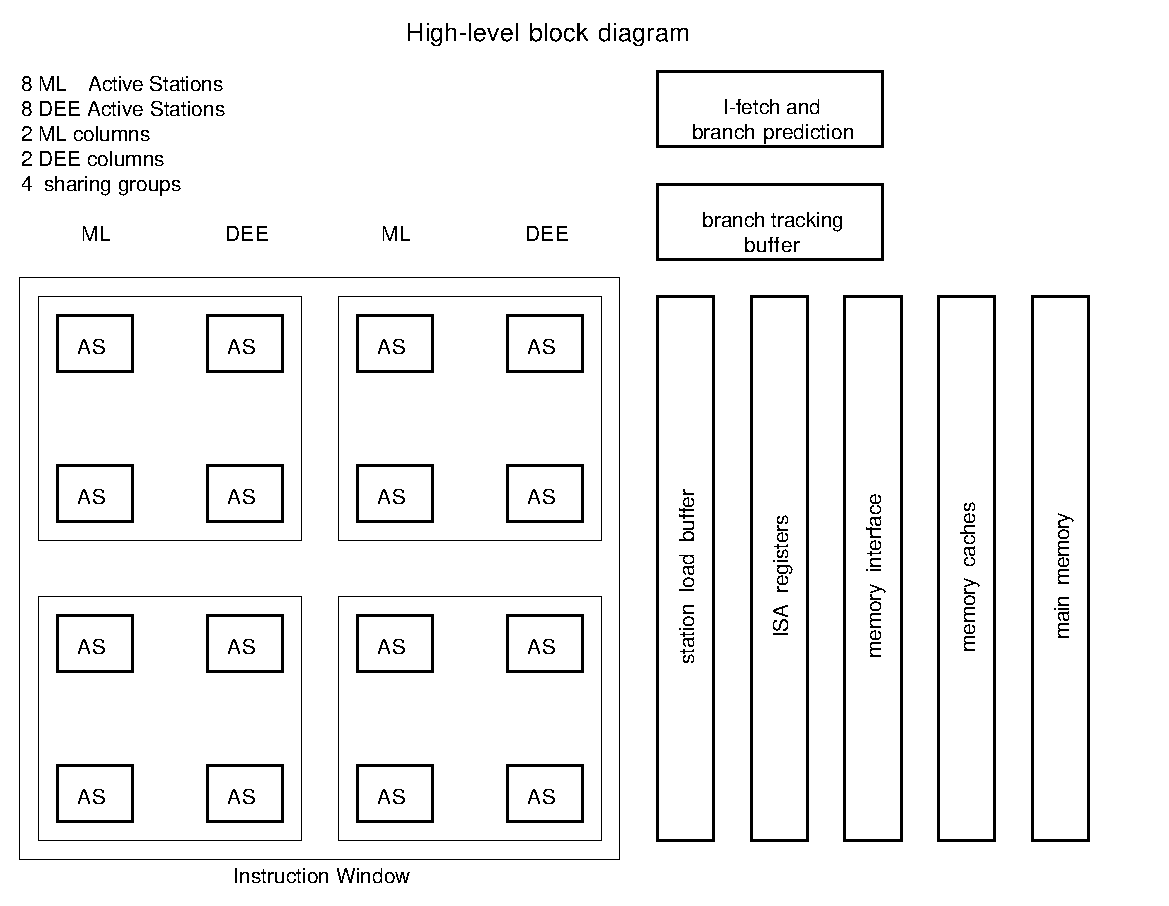
\epsfig{file=high.eps,width=4.0in}
\caption{{\em High-level View of the Distributed Microarchitecture.} 
Shown are the major hardware components of the microarchitecture.
With the exception of the 
execution window block, this is similar to most conventional
microarchitectures}.
\label{fig:high}
\end{figure}
%
Our microarchitecture shares many basic similarities to most conventional
machines.
The main memory block (usually the system DRAM),
the L2 cache (unified in the present case), and the L1 instruction 
cache are all rather identical to what is commonly used.
Except for the fact that the main-memory, L2 cache, and L1 data
cache are all address-interleaved, there is nothing further
unique about these components.  Our L1 instruction
cache is presently not address-interleaved.
The interleaving of memory, a common technique, provides an easy way
to substantially increase the bandwidth throughout the
memory system.  
The component labeled \textit{execution window} is where
our microarchitecture differs substantially from existing machines.
This component is discussed in more detail later.

Our L1 data cache is similar to
most conventional data caches except that it also has the ability to
track speculative memory writes.
Our L1 d-cache shares a similar goal with the 
Speculative Versioning Cache \cite{Gop98} 
but is simpler is some respects.
We allow speculative memory writes to propagate
out to the L1 data cache.  Multiple copies
of a speculative write may be present within the L1 data cache
at the time.  They are differentiated from each other
through the use of time-tags.  Time-tags are the basic mechanism
used in the microarchitecture to order all operands, including
memory operands, while they are being used by instructions
currently being executed.
More information on both the L1 data cache and the whole of
the memory subsystem in general is given in a report
by Uht \cite{Uht02b}.

The i-fetch unit first fetches instructions from i-cache
along one or more predicted program paths.
Due to our relatively large instruction fetch bandwidth
requirement, we allow for the fetching of multiple i-cache
lines in a single clock.
In our microarchitecture, instructions are immediately
decoded after being fetched.
All further handling of the instructions is done in their decoded
form.
Decoded instructions are then staged
into an \textit{instruction load buffer}
so that they are available to be loaded into the execution
window when needed.  
For this microarchitecture, we term the
transfer of decoded instructions from this buffer to our adaptation of
reservation stations to be \textit{instruction load}.
This instruction load buffer is organized so that
a large number of instructions can be broadside loaded into the
execution window in a single clock.
The multiple buses going from the i-fetch unit to the
execution window in Figure \ref{fig:high} is meant to
reflect this operation.  
Six buses are shown in that figure
as an example, but larger numbers are more likely in
realized machines.
The number of buses shown, illustrates the
number of instructions that can be simultaneously loaded for execution 
in a single clock of the machine.  
This number is also later referred to as 
the \textit{column height} of the machine.  

The execution window component 
represents the major departure of our microarchitecture
from all previous and existing ones.
Calling this part of the machine a component is actually somewhat
misleading since it is the majority of the hardware resources
for the whole of the microarchitecture.
The execution window will contain all of the instructions
that are being executed at any given time.  
This may be an
exceedingly large number as compared with 
existing conventional microarchitectures.
Due to the size and complexity of the execution window, it is
discussed in much more detail in the next section.
%
\subsection{The Execution Window}
%
Instructions within the execution window may be both actively 
executing
or may be waiting to be re-executed when events indicate that
a re-execution is warranted or required for proper program order
fulfillment.
Figure \ref{fig:window} shows a more detailed view
of the execution window.
This view is still at something of a high level but serves to
illustrate the main subcomponents with it.
The i-fetch unit is shown again on the far right as a reference.
%
\begin{figure}
%\vspace{0.2 in}
%\setlength{\epsfxsize}{10cm}%7
%\centerline{\epsfbox{window.eps}}
\centering
\epsfig{file=window.eps,width=5.8in}
\caption{{\em High-level View of the Distributed Microarchitecture.} 
Shown is a layout of the Active Stations (AS) and Processing Elements (PE)
along with some bus interconnections to implement a large,
distributed microarchitecture.}
\label{fig:window}
\end{figure}

We have extended the idea of Tomasulo's reservation
station \cite{Tom67} to provide the basic building block for a distributed
microarchitecture.  Tomasulo's reservation station provided for the
simultaneous execution of different instructions over several
functional units.  
Register results from the functional units were placed on
a common data bus and looped back to provide source register operands 
for instructions waiting in the reservations stations as well as
for updating of the register file.  In our microarchitecture,
an output result is not looped back to the input of the same reservation
station
that provided the result but rather is forwarded to different
stations that are spatially separated, in silicon or circuit board space,
from the first.  
This operation is termed \textit{operand forwarding}.
We (like others)
also extend the idea of the reservation station to allow for multiple
executions (re-executions) of the same instruction in the station.  We
keep instructions in their associated stations until they are
retired (either committed or squashed).  We call our adaptation of the
reservation station the \textit{active station} (\textit{AS}).
Like a reservation station, an active station can only hold a single
instruction at a time.  After an instruction is loaded into
as AS, it remains there until it can be retired from the execution
window.

Rather than lay the active stations out in silicon simply next to
function units that will execute the instructions loaded to them
(like with the original reservation station idea),
we lay them out in a two dimensional grid whereby sequentially
loaded instructions will go to sequential ASes down a column of
the two dimensional grid of ASes.  
The use of a two dimension
grid simply provides a means to implement the necessary
hardware either in a single silicon IC or through several
suitable ICs laid out in the grid on a circuit board.
The number of ASes in the height dimension of the grid is referred to
as the column height of the machine, which was introduced
previously.
The example machine of Figure \ref{fig:high} had a column height of
six due to the six buses that were shown for the broadside loading of 
instructions into the execution window.
The column height can also be seen more clearly in 
Figure \ref{fig:window} when one counts the total
number of ASes that form a given column of ASes.

Dispersed among the active stations are associated execution
units.  An execution unit is represented in the figure as
a \textit{processing element} (\textit{PE}).  
PEs may consist of an unified all-purpose execution unit capable of
executing any of the possible machine instructions or more likely
consist of
several functionally partitioned units individually tailored
for specific classes of instructions (integer ALU, FP, or other).
The latter case is typical of most all machines today.
Groups of active stations along with their associated processing
element (PE) are termed a \textit{sharing group} (SG).  
They are termed sharing groups because the execution
resources within one of them can serve many ASes.
Sharing groups somewhat resemble
the relationship between the register file, reorder buffer,
reservation stations, and function units of most conventional
microarchitectures.  They have a relatively high degree of bus
interconnectivity between them, as conventional microarchitectures do.
In our case, the active stations serve the role of both the
reservation station and the reorder buffer of more conventional
machines.
The use of this execution resource sharing arrangement allows
for reduced interconnections between adjacent SGs.
Basically, only operand results need to flow from one sharing
group to subsequent ones.
The transfer of a decoded instruction, along with its associated operands,
from an AS to its PE is isolated to within the given SG.

Referencing again the example machine layout
of Figure \ref{fig:window}, it can be seen that the example machine
shown consists of two columns of SGs.  
In our present microarchitecture, we always have two 
columns of ASes within a SG.
The first AS column within a SG is
reserved for the primary predicted speculative
execution path of the program.  
This AS column is labeled \textit{ML}
in the figure for \textit{main-line} path.
The second column of ASes is reserved for the possible
execution of a DEE path of the program and is labeled as such
in the figure..
In this machine example, each SG also contains three rows of ASes
and a single PE.
The ratio of AS rows to PEs in the SGs (all SGs
are configured the same) is, as expected, 
a primary performance metric of the microarchitecture.
Of course, most machines capable of substantial IPC
speedups will require larger, or much larger, numbers of
components than shown in the example of Figure \ref{fig:window}.
Typical machines explored so far have been in the
range of having eight or more SGs per column, each
with as many as sixteen or more AS rows per sharing
group, and as many as eight to 32 or more columns of SGs.
We generally characterize
a basic machine according to the tuple: 
%
\begin{itemize}
\item{sharing group rows}
\item{active station rows per sharing group}
\item{sharing group columns}
\item{maximum number of alternative speculative execution paths allowed}
\end{itemize}   
%
These four characteristic parameters of a given machine
are greatly influential to its performance 
and form a basic configuration on which experiments
are performed to explore other aspects of the machine.
We refer to these four parameters as the \textit{geometry} 
of a given machine.
We normally show these four numbers concatenated,
so if we assume that the example machine of the figure
is allowed to have as many as three
additional speculative execution paths (besides the predicted one),
then it would be abbreviated {\tt 2-3-2-3}.

The less bold horizontal buses (referencing Figure \ref{fig:window})
form the paths by which instructions are loaded to active stations
from the decoded instruction load buffers discussed previously.
These buses are unidirectional and can be, and typically are,
buffered at desired spatial intervals to provide 
scalability in the horizontal dimension
of the execution window.
Again, the instruction fetch unit is responsible for
fetching instructions from the memory hierarchy, these are then decoded
and placed into the load buffers.   

Also employed within the execution window is a scheme to
dynamically predicate, at execution time, 
all instructions that have been loaded
into active stations.  
This predication scheme essentially provides for each loaded instruction
an \textit{execution predicate}.  These execution predicates
are just a single bit (like with explicit architectural predication)
but are maintained and calculated within the microarchitecture
itself and are thus not visible at the ISA level of abstraction.
%
\subsubsection{Operand Forwarding and Machine Scalability}
%
An interconnect fabric is provided to forward result
operands from earlier ASes to 
later ASes, in program order.  
Result operands consist of the register, memory, and
instruction execution predicates that were discussed previously.
This interconnect allows for arbitrary numbers of sharing
groups to be used in a machine while still keeping all bus
spans to a fixed (constant length).
The interconnect fabric is simply shown by
the bold (primarily vertical) buses in 
Figure \ref{fig:window}.
There is not necessarily one type of interconnection
fabric possible for the forwarding of operands (of any of the
three types)
and we have explored several
different types and methods of operand forwarding already.
In the general case, several buses are used in parallel to make up
a single forwarding span.
This is indicated by the use of the
bold lines to depict the operand forwarding buses of the figure.  
More than one
bus in parallel is generally required to meet
the bandwidth needs of the machine.
Our present work uses four buses in parallel to make up
each of the forwarding bus spans needed.

Active bus repeater components are used (and required) to 
maintain constant bus spans, needed for scalability.
A bus repeater component is generally termed a
\textit{forwarding unit} (FU) and is labeled as such in the figure.
These forwarding units do more than just repeat operand values from
one span of a bus to the next.
For registers and memory, operands are filtered so that
redundant forwards of the same value (as compared with that last forwarded)
are eliminated.  These can also be termed \textit{silent forwards}.
This filtering provides a means to reduce the overall bandwidth
requirements of the forwarding interconnection fabric.
Each forwarding unit employed in the present work also has a small
amount of storage for memory operands.
This storage serves as a cache for memory operand values.
We term this small cache storage a \textit{L0 data cache}.

In this paper, we present just two of several methods that
may be possible for the forwarding of any of the three types of
operands (register, predicate, and memory).
We use one method for the forwarding of register and predicate
operands and a second method for the forwarding of memory 
operands.  Presently, the forwarding of operands partly share common
buses,
but buses can also be functionally separated.  
That is, for example, one or more buses could serve for
just register
forwarding while other buses could serve for memory and predicate forwarding.
We have yet to explore all of the alternatives.

For register and predicate operands, values that are generated
by ASes contend for one of the outbound buses
(labeled \textit{shared operand forwarding buses} in the figure) 
to forward the value.
Requests for bus use will be satisfied with any bus clock-slot that may be
available on any of the buses in parallel, belonging to
a given span.  All other ASes on the outbound bus span snoop
operand values forwarded from previous (in program order)
ASes.  In addition, a forwarding unit (the bus repeater) also
snoops the same operands and forwards the operand value to the
next bus span if necessary (the value was different than the previous
value).  For register and predicate operands, they are also
looped around from the bottom on one column of SGs
to the top of the next column of SGs.  
Operands from the bottom of the
far right column of SGs gets looped around to the
top of the far left column.  
This behavior forms the characteristic ring pattern of operand flow,
inherent in many microarchitectures.  Forming a closed loop
with these buses, and essentially just renaming columns (identifying the
one closest to retirement), is easier than physically transferring
(shifting) the contents of one column to the next when a column
of ASes retires.

For memory operands, we employ a second operand forwarding strategy.
When memory operands are generated by ASes, again the AS contends
for one of the outbound buses 
(labeled \textit{shared operand forwarding buses} in the figure) 
in order to forward the operand value.
However, unlike the register and predicate operand forwarding
strategy, memory operands also travel backwards, in program ordered
time, and get snooped by the forwarding units that are at the top
of each SG column.  This is done so that the operand can
be transfered onto a \textit{memory operand transfer bus}, shown
at the top of Figure \ref{fig:window}.  
These buses are address-interleaved and
provide the connectivity to get memory operands (generally
speculative) over to the L1 data cache.
They are tentatively stored in the L1 data cache along with 
their associated operand
time-tags until a committed value is determined.
Similarly, operands returning from the L1 data cache to service requests
from ASes, are first put on one of the memory operand transfer buses (based
on the interleave address of the operand).  These operands then get snooped
by all of the forwarding units at the top of each SG
column after which the operand is forwarded on a shared operand
forwarding bus to reach the requesting ASes.

Persistent register, predicate state and some persistent
memory state is stored in the forwarding units.
Persistent state is not stored indefinitely in any single forwarding
unit but is rather stored in different units as the machine
executes column shift operations (columns of ASes get retired
and committed).  However, this is all quite invisible to the ISA.
Exceptions in program flow (caused by the execution
of an instruction) are handled similarly to how they
are handled in any speculative machine.  Speculative exceptions
are held pending until they would be committed as determined
by all preceding conditional branches being resolved.
They are then handled as if an unconditional jump was encountered,
vectoring architected control flow off to an exception handler.
Subsequent program code would then save registers, as normally
would be done, without
knowledge of the underlying microarchitecture.
Interrupts can be handled in more flexible ways than exceptions.
One way to handle interrupts is to allow all instructions
currently being executed within the execution window to reach
commitment, then architected program flow can vector off to
a handler as if an unconditional jump was encountered, proceeding
as with the case of instruction execution exceptions above.
%
%
\subsection{Basic Machine Operation}
%
Instructions are fetched from memory, decoded, and staged in 
load buffers.
When an entire column
of ASes is free to accept new instructions, generally
an entire column of instructions are loaded to the free AS
column from the load buffer.  
Conditional branches are
predicted at or just before they are entered into the load buffers
(for subsequent load to the ASes).
The prediction of the branch 
is sent along with the
decoded instruction information when instructions are 
loaded to ASes.

All of the ASes in a given column are loaded with 
instructions in a single clock.  
In our present implementation, newly loaded instructions
are only loaded to a single column of ASes within
a column of SGs.  The other column of ASes 
in our current SGs (which currently have a total
of two columns of ASes) is reserved for the possible spawning of 
additional execution paths as a result of a condition branch instruction.
When and how additional paths are spawned is discussed later.

There are several strategies for
loading instructions to available AS columns.
Since all loaded instructions are speculative, instructions
from either outgoing path of a conditional branch can be loaded
to sequential ASes.
The fetch unit is responsible for preparing for such decisions.
Even when a conditional branch is predicted as being taken,
instructions may still be loaded to successive ASes following the not-taken
output path under most circumstances.  
If the distance to the target of a branch
that is predicted to be taken, is not too large (the more usual case),
instructions are loaded to ASes along the program \textit{static} order 
(or not-taken
path) of the branch in the hopes of capturing hammock styled branch
constructs.  A more detailed discussion on these alternatives is
presented in the next section.

Program dependencies (control, register, and memory) are 
maintained through the use of time-tags.
Time-tags are associated with all transient operands within the machine.
This has some resemblance to register tags used in more conventional 
microarchitectures but has been more generalized for use in this
distributed microarchitecture.  Instructions remain in their
associated ASes until they are retired by either being
committed or abandoned (squashed).  In this way, the ASes
(or rather the whole set of them)
fulfill the role of the reorder buffer or register update unit of more
conventional microarchitectures.
As a column of ASes get retired, that column becomes available
for the loading of newly decoded instructions from the load buffer.
Further, the time-tag values, associated with all transient operand
values in the machine, get decremented.
When the time-tag values of all operands gets decremented,
this is effectively a renaming of them.
The next column in the machine (that column with the next higher
time-tag values) also becomes the next column that will
get retired.
The operation of decrementing the time-tags associated with
the transient operands in the execution window is termed a \textit{column
shift}, for historical reasons.  
The hardware used for the snooping of an input operand of an AS
is shown in Figure \ref{fig:source}.
Basically, a new operand is snarfed when it has the same address and
path identifier as the current AS as well as
a time-tag value that is less than that of the current AS
but greater or equal to that of the last snarfed operand.
Simpler snooping hardware is used in forwarding units.
%
\begin{figure}
%\vspace{0.2 in}
%\setlength{\epsfxsize}{14cm}%7
%\centerline{\epsfbox{source.eps}}
\centering
\epsfig{file=source.eps,width=4.0in}
\caption{Operand Snoop Logic Within an AS.
The logic used for snooping of input operands for ASes
is shown.}
\label{fig:source}
\end{figure}
%

Much more detailed information about this microarchitecture
can be found in a technical report by Uht et al~\cite{Uht01}.
Additionally, a more detailed discussion of the mechanism used for
enforcing program dependencies in this microarchitecture
can be found in a report by Kaeli et al~\cite{Kaeli01}.
A more detailed discussion about multipath execution and
the spawning of DEE paths is given in the following section.
%
%
\subsection{Conditional Branches and Multipath Execution}
%
There are two major choices the machine needs to constantly
consider with regard to the handling of conditional branches at
execution time.
The first is whether to load instructions to sequential
ASes following
the not-taken path of the condition branch or to load instructions
along the taken path.  
The second major decision to make is
whether to spawn a DEE path
on any given conditional branch.

First, if a backward branch is predicted taken,
we will speculatively follow it and continue loading instructions
into the execution window for the mainline path from the target
of the branch.  
This case allows for the capture of program loops
within the execution window of the machine and can be thought of
as hardware loop unrolling.
For a backward branch that
is predicted not-taken, we continue loading following the
not-taken output path.

If a forward branch has a near target (small domain size) such
that it can be loaded within the execution window, 
then we
load instructions from the domain of the branch (following the
not-taken output path) whether or not it is the predicted path.
This represents the fetching of instruction in the 
memory or static order rather than the program dynamic order and
is very common in the absence of a loop.
Our mainline path continues along the predicted branch output path
regardless of whether it was the taken or not-taken one.  
We spawn a DEE path
for the opposite output of the branch from
the mainline path case, whatever it is.

For forward branches with a far target,
if the branch is predicted taken, we load instructions following the target
of the branch.  If the branch is predicted not-taken, we continue
loading instructions for the mainline path following the not-taken
outcome of the branch.  In both of these cases, we do not
spawn a DEE path for this branch.

DEE paths are created by loading an available
column of ASes, a free second column of ASes within a SG column, with
the same decoded instructions from the AS column that contained
the conditional branch instruction that gave rise to the DEE path.
As mentioned previously, the second column of ASes in each sharing
group column is reserved for DEE paths.
However, there are still a limited number of these AS columns
available at any one time in the machine.
Several strategies for the management of these AS columns is
possible and we present two such strategies in the present work.

One such strategy is very simple and just 
spawns DEE paths for suitable conditional
branches (as explained above) on a first come, first served basis.  
That is, as machine
execution resources that are reserved for DEE paths
becomes available, those resources are assigned to the next conditional
branch for which an DEE path has not already 
been assigned.  The DEE path is allowed to
remain executing until its originating conditional
branch get resolved (at which point its DEE
path is squashed).
This is a simple strategy but might
not give the best IPC speedups as compared with more complicated
strategies.  

A second strategy that we explore, is to monitor
the amount of time that existing DEE paths have been
resident in the execution window, and to squash those paths that
have reached a residency threshold.  Residency time in the
execution window is approximated by the number of column shifts that
have occurred since a DEE path was spawned.  
Again, a column
shift corresponds with the retirement of the AS column with the
lowest numbered time-tags (toward the value zero).
The rationale is that the longer a DEE path is resident
within the execution window,
the likelihood of the conditional branch that gave rise to it being 
mispredicted becomes less.  
Thus, that DEE path is no longer using the
underlying execution resources as well as maybe some new DEE
path might.
When a DEE path is 
squashed in order to make room for
the spawning of a new DEE path, the associated
executed resources are released for assigned to another conditional
branch.
We term this the \textit{release} strategy of managing
DEE paths.
%
%
\section{Simulation Results}
%
We present results from simulations of a set of machine geometries
using the general microarchitecture described previously.
We first describe our simulation process.
We them present two major sets of results.
The first major set of results shows program IPC for each of three
modes of execution of the machine.
The second major results shows the sensitivity of our machine
to varying the latencies of several components in the memory hierarchy.
%
\subsection{Methodology}
%
The simulator is a recently built tool that shares some similarity
to SimpleScalar \cite{Austin97} but which was not based on it.
We execute
SpecInt-2000 and SpecInt-95 programs on a simulated machine
that features a MIPS-1 ISA along with the addition of some MIPS-2 and
MIPS-3 ISA instructions.  We are using the standard SGI Irix system
libraries so we needed to also support the execution of some
MIPS-2 and MIPS-3 instructions to accommodate
that.  All programs were compiled on an SGI machine under the
Irix 6.4 OS and using the standard SGI compiler and linker.  
All benchmark programs were compiled with
standard optimization ({\tt -O}) for primarily the MIPS-1 ISA ({\tt -o32}).
No changes to the SGI compiler or linker were made to create
the binary benchmark programs.

For our benchmark programs, we chose five programs to work with,
four from the SpecInt-2000 benchmark suite
and one from the SpecInt-95 program suite.
These programs were chosen to get a range of different memory and looping
behavior while keeping the number of programs to be simulated small.
The particular programs used along with some statistics 
are given in Table \ref{tab:benches}.
All programs were executed using the SpecInt reference inputs.
All accumulated data was gathered over the simulated execution of
500 million instructions,
after having skipped the first 100 million instructions.
The first 100 million instructions, however, were used to warm up the
various simulator memory caches.
%
\begin{table}
\begin{center}
\caption{Benchmarks Programs Simulated and Some Statistics.}
\label{tab:benches}
\begin{tabular}{|l|c|c|c|c|c|}
\hline 
benchmark&bzip2&parser&go&gzip&gap\\
\hline 
\hline 
br. prediction accuracy&90.5\%&92.6\%&72.1\%&85.4\%&94.5\%\\
\hline 
avg. L1-I hit rate&97.2\%&96.6\%&92.4\%&94.7\%&89.0\%\\
\hline 
avg. L1-D hit rate&98.8\%&99.0\%&98.8\%&99.8\%&99.3\%\\
\hline 
avg. L2 hit rate&90.1\%&86.0\%&96.8\%&73.0\%&88.5\%\\
\hline 
dynamic cond. brs.&7.0\%&13.0\%&9.0\%&8.8\%&6.2\%\\
\hline 
forward brs.&81\%&85\%&89\%&85\%&91\%\\
\hline 
S-S hammock brs.&23.4\%&42.1\%&35.7\%&45.2\%&27.3\%\\
\hline
\end{tabular}
\end{center}
\end{table}
%
The dynamic conditional branches in Table \ref{tab:benches} are
a percent of total dynamic instructions.
The numbers for the forward branches and the Simple Single-sided (S-S)
Hammock
branches are percentages of total dynamic conditional branches.
%
\subsection{IPC Results for Singlepath and Multipath Execution}
%
In this section, we present IPC data for five geometries
of the machine.  We have results for three different 
modes of 
machine execution.  These are : no multipath execution (singlepath),
simple multipath execution , and enhanced multipath execution.

The numbers of each of the major machine components, for each of the 
five
simulated geometries, are given in Table \ref{tab:configs}.
Although we have explored a large number of various sized
machines, these particular geometries were chosen in order
to get a range of IPC performance across a number of very
different machine sizes and shapes.
The common machine characteristics used in this section for
obtaining IPC results is given in Table \ref{tab:params}.
The L1, L2, and main memory access latencies do not include
the forwarding unit and forwarding bus delays within the
execution window.
The main memory latency is for a read to a new DRAM row.
These machine characteristics are fairly representative of
existing typical values.  Our choice for the main memory
access latency is somewhat conservative for an existing
1 GHz machine and might be typical of a 2 GHz CPU clock using
the fastest DDR-SDRAMs (33 nsec access times) and a custom or integrated 
DRAM interface controller.
Main memory performance is dominated
by DRAM technology and major improvements in speed for high volume
devices are not soon
expected over the current fastest devices \cite{Sam99},
thus making conservative estimates somewhat appropriate.
%
\begin{table}
\begin{center}
\caption{Machine geometries simulated for each of the benchmark
programs.}
\label{tab:configs}
\begin{tabular}{|c|c|c|c|}
\hline 
SG rows&
ASes per SG&
SG columns&
max D-paths\\
\hline
\hline 
8&4&8&8\\
\hline 
8&8&8&8\\
\hline 
16&8&8&8\\
\hline 
32&2&16&16\\
\hline 
32&4&16&16\\
\hline
\end{tabular}
\end{center}
\end{table}
%
\begin{table}
\begin{center}
\caption{General machine characteristics.}
\label{tab:params}
\begin{tabular}{|l|l|}
\hline 
L1 I/D cache access latency&1 clock\\
\hline
L1 I/D cache size&64 KBytes\\
\hline
L1 I/D block size&32 bytes\\
\hline
L1 I/D organization&2-way set associative\\
\hline
L2 cache access latency&10 clocks\\
\hline
L2 cache size&2 MBytes\\
\hline
L2 block size&32 bytes\\
\hline
L2 organization&direct mapped\\
\hline
main memory access latency&100 clocks\\
\hline
memory interleave factor&4\\
\hline
forwarding unit minimum latency (all)&1 clock\\
\hline
forwarding-bus latency (all)&1 clock\\
\hline
number of forwarding buses in parallel&4\\
\hline
\end{tabular}
\end{center}
\end{table}
%
The IPC results for each of the three modes of machine execution
are presented in Tables \ref{tab:ipc1}, \ref{tab:ipc2}, and \ref{tab:ipc3}.
The geometry labels (4-tuples) 
at the tops of these tables consist of the concatenated 
numbers of
machines components for: SG rows, AS rows per SG, SG columns,
and the maximum DEE paths allowed for that execution.
For each table we also present the IPC results for each program
(except GAP for which we had simulation difficulties) on a baseline
conventional superscalar machine.  The conventional machine was
simulated using SimpleScalar \cite{Austin97} using the PISA
instruction set (a MIPS-like instruction set) and 
used a machine configuration that
matched as closely as possible the various parameters listed
in Table \ref{tab:params} above.  
The IPC results from SimpleScalar
serve as a baseline for comparison and are repeated, and
labeled \textit{baseline}, in each of the results.

Table \ref{tab:ipc1} gives the IPC results for each of the benchmark
programs over various machine geometries, when executing in
singlepath mode.
For this singlepath execution case,
the maximum number of DEE paths allowed is zero (as indicated).
In addition to the individual benchmark IPC results, we also
present the harmonic mean of the IPC across all benchmarks.
Table \ref{tab:ipc2} gives the results using the simple method 
(first-come-first-serve) for
the spawning of DEE paths.
%
\begin{table}
\begin{center}
\caption{IPC results for singlepath execution.}
\label{tab:ipc1}
\begin{tabular}{|c|c|c|c|c|c|c|}
\hline 
geometry&baseline&
8-4-8-8&
8-8-8-8&
16-8-8-8&
32-2-16-16&
32-4-16-16\\
\hline 
\hline
bzip2&2.0&3.4&4.2&4.8&4.2&4.7\\
\hline 
parser&1.8&2.9&3.3&3.8&3.5&3.9\\
\hline 
go&1.7&2.6&3.2&3.7&3.4&3.6\\
\hline 
gzip&1.6&3.4&4.4&5.2&4.8&5.3\\
\hline 
gap&-&4.5&5.6&6.1&6.5&6.3\\
\hline
\hline 
HAR-MEAN&1.8&3.2&4.0&4.6&4.2&5.6\\
\hline
\end{tabular}
\end{center}
\end{table}
%
\begin{table}
\begin{center}
\caption{IPC results for simple multipath execution.}
\label{tab:ipc2}
\begin{tabular}{|c|c|c|c|c|c|c|}
\hline 
geometry&baseline&
8-4-8-8&
8-8-8-8&
16-8-8-8&
32-2-16-16&
32-4-16-16\\
\hline 
\hline 
bzip2&2.0&3.9&4.8&5.5&4.9&5.3\\
\hline 
parser&1.8&4.0&4.3&5.1&5.6&5.1\\
\hline 
go&1.7&4.6&5.6&6.4&6.0&6.3\\
\hline 
gzip&1.6&4.7&5.9&6.8&6.2&6.8\\
\hline 
gap&-&5.6&6.9&7.1&8.3&7.2\\
\hline 
\hline 
HAR-MEAN&1.8&4.5&5.4&6.1&5.8&6.1\\
\hline
\end{tabular}
\end{center}
\end{table}
%

Examining the data, we can see that our simple 
(first-come-first-serve)
multipath execution
strategy significantly outperforms singlepath execution.
This was expected as our microarchitecture is able to
capture many forward conditional branch domains inside the execution
window and speculatively execute both outcomes of these branches
as a bet against a misprediction.

Next we want to get results for machine simulations using our
more complicated \textit{release} management strategy for DEE paths.
In this enhanced strategy, DEE paths are allowed to
remain within the execution window for a certain number of
columns shifts (described previously).  We first attempt to
determine the best number of column shifts to use as a metric
for path residency.  For this we took one machine geometry and
varied the number of column shifts the machine waits before releasing
a DEE path.
We use the machine geometry of 16-8-8-8 along with the parameters
listed in Table \ref{tab:params}
to investigate
IPC speedups as the number of column shifts waited for is varied.
Figure \ref{fig:release} shows the resulting IPC speedups,
as compared with the simple disjoint path management strategy.
%
\begin{figure}
%\vspace{0.2 in}
%\setlength{\epsfxsize}{14cm}%7
%\centerline{\epsfbox{release.eps}}
\centering
\epsfig{file=release.eps,width=4.0in}
\caption{Machine IPC speedup results for varying 
column shifts.}
\label{fig:release}
\end{figure}
%
For this particular machine geometry, this strategy
performs worse than the simple strategy when the number
of column shifts waited for is 
approximately fewer than four or five.
However, when DEE paths are retained in the
execution window for approximately
six columns shifts,
a performance speedup of about two to five percent is realized
over the simple DEE path strategy.
From these results, we will chose to allow DEE paths
to remain in the execution window for six column shifts
for all five machine geometries explored and all benchmarks.

Table \ref{tab:ipc3} gives the results using the \textit{release} 
method for the spawning of DEE paths.
Again, these allow DEE paths
to stay resident in the execution window through six column shifts
(determined above)
and the remaining parameters of the machine 
are those in table \ref{tab:params}.
%
\begin{table}
\begin{center}
\caption{IPC results for multipath execution using D-path release.}
\label{tab:ipc3}
\begin{tabular}{|c|c|c|c|c|c|c|}
\hline 
geometry&baseline&
8-4-8-8&
8-8-8-8&
16-8-8-8&
32-2-16-16&
32-4-16-16\\
\hline 
\hline
bzip2&2.0&4.2&5.0&5.8&5.4&5.7\\
\hline 
parser&1.8&4.3&4.6&5.3&5.0&5.4\\
\hline 
go&1.7&5.1&5.9&6.7&6.5&6.8\\
\hline 
gzip&1.6&5.0&6.3&7.0&6.7&7.2\\
\hline 
gap&-&6.0&7.5&7.5&8.9&7.9\\
\hline 
\hline 
HAR-MEAN&1.8&4.8&5.4&6.4&6.2&6.5\\
\hline
\end{tabular}
\end{center}
\end{table}

%
From these results, 
it is observed that our more complicated DEE \textit{release} strategy
performs better than our simple strategy for all machine
geometries explored here.
This is encouraging and suggests that attention to the
management of the DEE paths is important to getting
higher IPC speedups.
Some other strategies for the management of how and when to
spawn DEE paths have been proposed but they have not yet been
explored.  
This is an area that we intend to explore more
fully in the future.
%
\subsection{Memory Sensitivity Results}
%
In this section we present IPC data corresponding to varying some
parameters associated with the memory subsystem.
We show IPC speedup results for varying the access latencies,
in clocks, for: L1 I-cache,
L1 D-cache,
L2 cache, and
main memory.
All of this data was gathered on a machine geometry 
of 16-8-8-8 with the other parameters (the ones that are
not varied) being those that are listed in Table \ref{tab:params}.
Figure \ref{fig:l1icache} presents the speedups for varying
the L1 I-cache hit latency clocks from zero up to eight.
Figure \ref{fig:l1dcache} presents IPC speedup results
as the L1 D-cache hit latency is varied from zero clocks through to
eight clocks.
For these two figures, the speedups (the ordinate)
range from 0.9 through 1.2.
Figure \ref{fig:l2cache} presents the speedup results
as the L2 cache (unified I/D) hit latency is varied from 
zero clocks up to 16 clocks (our design choice was 10 clocks).
Finally Figure \ref{fig:dram} presents the IPC speedup results
as the main memory access hit latency is varied from twenty clocks 
up to 800 clocks.
For the L2 cache and DRAM sensitivity graphs, the speedups
(ordinate) range from 0.9 through 1.02.
All IPC speedups in these figures are relative to the zero
access latency cases.  The cases that have zero access latencies
still incur the various bus and active repeater delays that
are inside the execution window of the microarchitecture.
%
\begin{figure}
%\vspace{0.2 in}
%\setlength{\epsfxsize}{14cm}%7
%\centerline{\epsfbox{l1icache.eps}}
\centering
\epsfig{file=l1icache.eps,width=4.0in}
\caption{Machine IPC speedup results for varying 
L1 I-cache hit delay in clocks.}
\label{fig:l1icache}
\end{figure}
%
\begin{figure}
%\vspace{0.2 in}
%\setlength{\epsfxsize}{14cm}%7
%\centerline{\epsfbox{l1dcache.eps}}
\centering
\epsfig{file=l1dcache.eps,width=4.0in}
\caption{Machine IPC speedup results for varying 
L1 D-cache hit delay in clocks.}
\label{fig:l1dcache}
\end{figure}
%
\begin{figure}
%\vspace{0.2 in}
%\setlength{\epsfxsize}{14cm}%7
%\centerline{\epsfbox{l2cache.eps}}
\centering
\epsfig{file=l2cache.eps,width=4.0in}
\caption{Machine IPC speedup results for varying 
L2 cache hit delay in clocks.}
\label{fig:l2cache}
\end{figure}
%
\begin{figure}
%\vspace{0.2 in}
%\setlength{\epsfxsize}{14cm}%7
%\centerline{\epsfbox{dram.eps}}
\centering
\epsfig{file=dram.eps,width=4.0in}
\caption{Machine IPC speedup results for varying 
main memory access latency in clocks.}
\label{fig:dram}
\end{figure}
%
As can be seen from Figures \ref{fig:l1icache} and \ref{fig:l1dcache},
the machine is slightly more sensitive to L1 D-cache latency
than to L1 I-cache latency.  This is expected due to the
variability due to speculative memory accesses that is present for 
data memory accesses
that is not as prevalent in instruction accesses.
The GAP program appears less sensitive to L1 instruction or
data latencies and this is probably due to its looping
behavior that provides better spatial and temporal locality
for memory accesses.  Fortunately, latencies of 1 or 2 clocks
for L1 caches is more likely to scale better with increasing
processor clock than memory components further from the processor.

For the L2 cache (ours is currently unified), speedups are
possible when using short clock latencies than the 10 clocks that
we used as our default.
Although L2 latencies are likely to also scale somewhat
with future increasing processor clock rates, they are not likely
to scale as well as L1 is expected to do.
Fortunately our machine already gets good IPC performance
at the L2 cache latency of 10 clocks.

With respect to main memory (DRAM), the microarchitecture
is quite insensitive to latencies out to 100 clocks and
only then starts to degrade slightly after that.  
Since 100 clocks
(as we count it -- after our repeater and bus delays)
is probably typical at the present time (assuming a 2 GHz
CPU clock rate and the latest DDR-SDRAMs), our memory system
arrangement is properly hiding most of the long DRAM latency as it
should.  Since our machine is still quite insensitive to
main memory latency out to 800 clocks, we might expect to
operate the current machine up to about 10 GHz with similar performance.
Our insensitivity to DRAM latency is due to both the conventional
use of L1 and L2 caches but also to our use of L0 caches
within each of our bus repeater forwarding units.
Dispersing memory operand caches within our execution window
brings some memory storage very close to executing instructions
that use those memory operands.
%
%
\section{Conclusions}
%
We have presented the overview of a large-scale distributed 
microarchitecture suitable for extracting high ILP from
sequential programs.
This microarchitecture is designed to also implement 
speculative multipath execution.  We presented results
for the machine executing in singlepath mode and two types
of management for alternative speculative paths in multipath mode.
It was shown that multipath execution provides additional IPC
performance over singlepath execution using
both of the heuristics that we explored for
managing the alternative paths.
Further, our enhanced DEE path \textit{release} heuristic provided
an additional average of about five percent better IPC over the
simple DEE path management heuristic for a modest sized machine.
We also showed that our microarchitecture exhibits significant
insensitivity to a wide range of memory system component latencies.
%
\bibliographystyle{latex8}
\bibliography{high}
%
\end{document}
%
%
